\section{Method}
\label{sec:method}
In this section,
we utilized the {\it two-tier probability model} to calculate
the probability that the message can be received by the destination node
if the forward follows the specific path.
Furthermore,
we introduced the privacy preserving scheme to
protect the daily patterns of bicycle trips,
and then proposed the routing algorithm based on Dijkstra.

\subsection{Delivery Metric Calculation based on Probability Model}
\label{subsec:r_metric}
Considering that the discrete probability density function in (\ref{eq:prob_seq})
can only provide that the probability of the $1$-hop forwarding,
we will propose the delivery metric based on the integral methodology
to estimate the probability that the message arrives at the destination node
along the specific path before the lifespan exhaust.

Assume that a contact $i \rightarrow j$ occurs at time $t$.
A $3$-hop potential routing path $<j, r_{1}, r_{2}, d>$ needs to be evaluated.
$i$ is the node that carries the message until now.
$j$ is the potential message carrying node,
which may forward the message to the destination sooner.
$d$ is the destination node of the message.
$r_1$ and $r_2$ is the potential relay node.
If the message can be delivered following the path $<j, r_{1}, r_{2}, d>$,
the contact sequence should occur at least once
before the message lifespan exhausts��
which means that the $3$ contacts
$i \rightarrow r_1$, $r_1 \rightarrow r_2$, $r_2 \rightarrow d$
occurs one after another in the future at least once.
Let $t$ denote the current time.
$T$ is the time when the lifespan of the forwarded message exhausts,
i.e., the deadline of receiving this message.
Then the delivery probability can be calculated as
\begin{equation}
\label{eq:G_continuous}
g^{t, T} = \int_{t}^{T} {f}_{i,r_1}(\tau_0)
\int_{\tau_0}^{T} {f}_{r_1, r_2}(\tau_1)
\int_{\tau_1}^{T} {f}_{r_2, d}(\tau_2)
\mathrm{d} \tau_2 \mathrm{d} \tau_1 \mathrm{d} \tau_0,
\end{equation}
where ${f}_{i,r_1}(\tau_0)$ denotes the continuous probability density function
that $i \rightarrow r_1$ occurs at the time $\tau_0$.
Similarly, both ${f}_{r_1, r_2}(\tau_1)$ and ${f}_{r_2, d}(\tau_2)$
are the continuous probability density function
of the corresponding contacts.
To mitigate the computation burden of the continuous integral
in (\ref{eq:G_continuous}),
we can utilize the probability sequence in $(\ref{eq:prob_seq})$.
Thus we can transform the integral in (\ref{eq:G_continuous})
into the discrete summation, which is
%compute the routing metric of $<r_{0}, r_{1}, r_{2}, d>$ at time $t$ as
%old version of discrete G
%\begin{equation}
%\label{eq:G_discrete}
%g^{t, T} = \sum_{\tau_0 = t}^{T-2} \left( q_{i, r_{1}}^{\tau_0} \times
%\sum_{\tau_1 = \tau_0 + 1}^{T-1} \left( q_{r_{1}, r_{2}}^{\tau_1} \times
%\sum_{\tau_2 = \tau_1 + 1}^{T}  q_{r_{2}, d}^{\tau_2} \right) \right).
%\end{equation}
\begin{equation}
\label{eq:G_discrete}
g^{t, T} = \sum_{\tau_0 = t}^{T} \left( q_{i, r_{1}}^{\tau_0} \times
\sum_{\tau_1 = \tau_0}^{T} \left( q_{r_{1}, r_{2}}^{\tau_1} \times
\sum_{\tau_2 = \tau_1}^{T}  q_{r_{2}, d}^{\tau_2} \right) \right),
\end{equation}
where $q_{i, r_{1}}^{\tau_0}$ denotes the $\tau_0$th term in the probability sequence $seq_{i, r_{1}}$.
Similarly, we can obtain $q_{r_{1}, r_{2}}^{\tau_1}$ and $q_{r_{2}, d}^{\tau_2}$.
Here $t$ and $T$ have been converted into
the indices of the probability sequence
$0,1,\cdots,24T_m-1$.

With the probability sequence and (\ref{eq:G_discrete}),
we can calculate $g^{t, T}$ of every path from $j$ to $d$ and from $i$ to $d$.
$1$)If the maximal $g^{t,T}$ from $j$ to $d$
is higher than the maximal $g^{t,T}$ from $i$ to $d$,
$j$ is the better relay node than $i$.
Then the message should be forwarded to $j$ upon this contact.
$2$)Otherwise, the message should be stored in $i$
until the next contact.
However, the computation burden of the scheme
based on (\ref{eq:G_discrete}) is considerable.
Assume there are $L$ hours from $t$ to $T$.
The number of terms $q \times q \times q$ is
$\sum_{l=1}^{L} + \sum_{l=1}^{L-1} + \cdots + \sum_{l=1}^{2} + 1 \le L^3$.
Moreover, in order to justify whether $i$ is a better relay node than $j$,
we will calculate $g^{t,T}$ of all the pathes
from $i$($j$) to $d$ to get the maximal one.
If the path search process is based on BFS (Breadth-First Search),
the computation complexity is $O(N^h L^h)$, where $h$ is the search depth.
That means that the scheme based on the path search
and the path evaluation will lead to the heavy computational burden.
And this scheme based on $g^{t,T}$ is not proper
in the BSS-OppNet scenario.
%all the possible path should be obtained before be evaluated.

\begin{figure}
  \centering
  {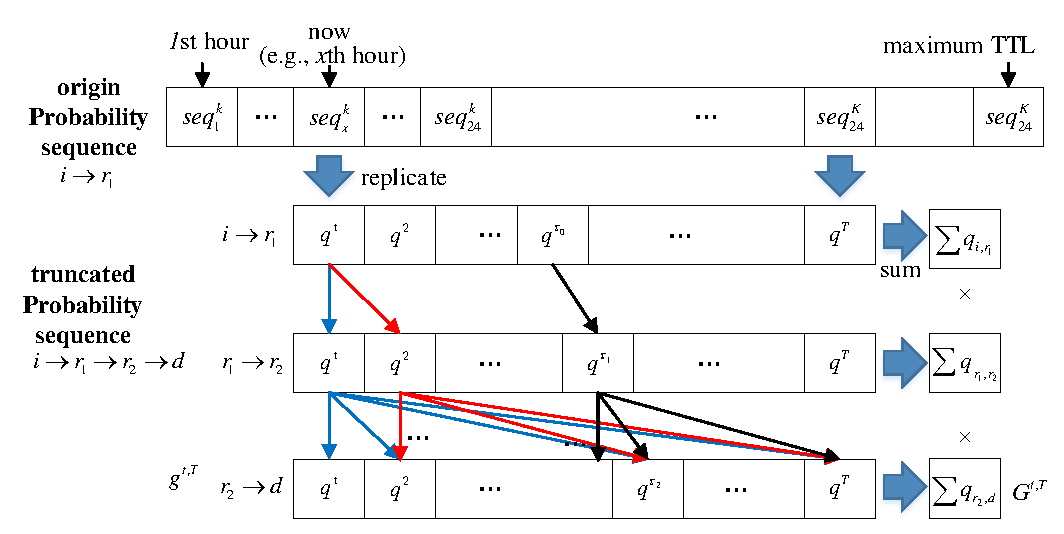
\includegraphics[width=0.47\textwidth]{fig/deliverymetric.eps}}
     \caption{Calculation of $g^{t,T}$ and $G^{t,T}$.}
     \label{fig:g_G}
\end{figure}
%[
%Maybe we can Reduce Matrix, less than 0? delete and pull the after ones!
%!!!
%Currently, we introduce a simple method to represent the routing metric,
%which is
%\begin{equation}
%G^{t, T} = \sum_{h=0}^{T-2-t_0} \sum_{\tau = t_0}^{T-2-h}
%seq_{r_{0}, r_{1}}^{\tau} seq_{r_{1}, r_{2}}^{\tau+1} seq_{r_{2}, d}^{\tau+2}
%\end{equation}
%The performance is good, but is not consistent
%with (\ref{eq:G_continuous}) and (\ref{eq:G_discrete}).
%]
In order to reduce the computation burden of the delivery probability in (\ref{eq:G_discrete}),
we can also the approximate metric of the path from $i$ to $d$, which is,
\begin{equation}
\label{eq:G_origin}
G^{t, T}_{i,d} = \sum_{\tau_0 = t}^{T} q_{i, r_{1}}^{\tau_0} \times
\sum_{\tau_1 = t}^{T} q_{r_{1}, r_{2}}^{\tau_1} \times
\sum_{\tau_2 = t}^{T} q_{r_{2}, d}^{\tau_2}.
\end{equation}
%whose computation complexity is $O(hn+h)$.
Fig.~\ref{fig:g_G} shows an example of calculating $g^{t,T}$ and $G^{t,T}_{i,d}$,
where the probability sequence is truncated based on the current time $t$
and the message lifespan $T$.
Take $<j, r_{1}, r_{2}, d>$ as an example,
we can find that these three summation,
i.e., $\sum_{\tau_0 = t}^{T} q_{i, r_{1}}^{\tau_0}$,
$\sum_{\tau_1 = t}^{T} q_{r_{1}, r_{2}}^{\tau_1}$
and $\sum_{\tau_2 = t}^{T} q_{r_{2}, d}^{\tau_2}$
are independent from each other.
Then we need to find the path with the maximal $G^{t, T}$
from all the pathes from $i$ to $d$.
Note all the summations, including $\sum_{\tau_0 = t}^{T} q_{i, r_{1}}^{\tau_0}$,
$\sum_{\tau_1 = t}^{T} q_{r_{1}, r_{2}}^{\tau_1}$
and $\sum_{\tau_2 = t}^{T} q_{r_{2}, d}^{\tau_2}$, range from $0$ to $1$.
If we apply $\log_{a}$ in both sides of (\ref{eq:G_origin}),
and get,
\begin{equation}
\label{eq:log_sum}
\begin{aligned}
\log_{a} G^{t, T}_{i,d} =& \log_{a} \{\sum_{\tau = t}^{T} q_{i, r_{1}}^{\tau}\}
+ \log_{a} \{ \sum_{\tau = t}^{T} q_{r_{1}, r_{2}}^{\tau} \} \\
&+ \log_{a} \{ \sum_{\tau = t}^{T} q_{r_{2}, d}^{\tau} \},
\end{aligned}
\end{equation}
where $a \in (0,1)$, e.g., $a = 0.5$.
Then every term in (\ref{eq:log_sum})
ranges from $0$ to $+\infty$ and decreases with the summation term increasing.
Because that the path with maximal $G^{t, T}_{i,d}$ of all the pathes
denotes the delivery ability of the relay node,
the minimal $\log_{a} G^{t, T}_{i,d}$ is required to find out.

If all the nodes in OppNet are viewed as
the vertexes in the graph $G(\mathcal{N}, \mathcal{N} \times \mathcal{N})$.
Let the weight of the edge from $i$ to $i^{\prime}$
as $\log_{a} \{\sum_{\tau = t}^{T} q_{i, i^{\prime}}^{\tau}\}$.
The path weight is computed as
the weight summation of all the edges along the specific path.
Thus the problem of searching the maximum $G^{t, T}_{i,d}$
becomes the shortest path algorithm,
i.e., the search of the minimum $\log_{a} G^{t, T}$.
Note that all the weight is not less than $0$.
Therefore, we can use the classical Dijkstra algorithm
to find the path with the minimal $\log_a G^{t, T}_{i,d}$.
The graph is represented by the adjoint matrix.
The computation complexity of initializing the adjoint matrix
is $O(N^2L)$.
Thus the computation complexity of the scheme
based on (\ref{eq:log_sum}) is $O(N^2L)$.
%This formula implies that the search of the maximal $G^{t, T}$ is the search of $\log_{a} G^{t, T}$.
%the routing algorithm can be resolved by
%the shortest path algorithm (famous algorithms: Dijkstra? A*?).
%
%Furthermore, we compute the routing metric of the relay node.
%For example, we consider which of $i$ and $j$ is a better relay node
%for the message destination $d$ and TTL $T$.
%The depth first search of $i$ is conducted to obtain some potential paths,
%e.g., $<r_{0}, r_{1}, r_{2}, d>$, when we want to evaluate $i$.
%In order to reduce the number of valuable paths,
%the hop, whose corresponding $P_{ij}$ is less than $P_{th}$,
%should be ignored in the path search process.
%Then we compute $G_{t,T}$ for every path in the searched path set $\mathcal{P}$.
%And the maximum $G_{t,T}$ of $\mathcal{P}$ will be treated
%as the routing metric of relay node $i$.
%If $i \rightarrow j$ occurs,
%the message will be forwarded from $i$ to $j$
%only when $i$ can provide the higher $G_{t,T}$.

\subsection{Differential Privacy Preserving of Contact Pattern}
\label{subsec:dp}
Since the intra-day probability can reveal the context of the bike station in BSS,
the privacy of the contact pattern between two stations should be protected.
%ԭ��Ӧ����introduction ����
Take the contact $i \rightarrow j$ as an example,
%% i �� j ��Ӧ�ø��� ���㲥�Ŷԣ�
$\{p_{i, j}^x\}$ will be published from $i$ to all the contacted nodes for the future delivery metric computation.
However, the privacy of the relations between $i$ and other nodes, including $j$,
will be exposed simultaneously.
If most of trips from $i$ to other nodes occur around the commuting time in the morning on the weekdays,
$i$ can be inferred as the stations around the residential zones (e.g., station $210$ in Fig.~\ref{fig:intradayp}).
%If one node that is hacked has received $\{p_{i, j}^x\}$ ($i, j \in \mathcal{N}$),
%it may infer the context of $i$, e.g., the metro station (station $183$), the residential area (station $210$),
%which is shown in Fig.~\ref{fig:intradayp}.
%the hackers can infer that station (node) $210$ locates near the residential areas with much.
Moreover, the accurate $\{p_{i, j}^x\}$ may also reveal the history contacts, especially when the contacts are few.
For example,
if the difference between $\{p_{i, j}^x\}$ on July $1$st $2017$
and $\{p_{i, j}^x\}$ on July $2$nd $2017$ is $\Delta p_{i, j}^8 = 0.8$,
the malicious person ($Bob$) will infer there existed at least one contact from $i$ to $j$ around $8:00$ on July $1$st $2017$.
%���ͬʱP��С ����ȷ��ֻ��1��contact�����ڴ�ʱ
If $Bob$ knows that $Alice$ ride a bike at that time,
he can even predict the residential locations of $Alice$ around $i$.
Combing with these side information, the bike trip record, the identity of the bike user, 
and even the residential/affiliate location of user may be leaked
from the published $\{p_{i, j}^x\}$.

The differential privacy~\cite{Dwork14DP}, as a privacy preserving method with solid theoretical foundations,
can be employed to protect the released pattern.
One of widespread methods in differential privacy is the Laplace mechanism,
where the published $\{{p^{\prime}}^x_{i,j}\}$ will be obscured according to
${p^{\prime}}^x_{i,j} = p^x_{i,j} + Lap(\frac{\Delta f}{\varepsilon})$.
Here $Lap(\frac{\Delta f}{\varepsilon})$ is the probability density function of laplace noise with mean $0$.
Each element in the pattern vector $\{p^x_{i,j}\}$, e.g., $p^x_{i,j}$
should be added with a laplace noise.
$\varepsilon$ is the specified privacy parameter to
control the magnitude of privacy preserving.
Because $0 \le p^x_{i,j} \le 1$,
the maximum distance between two neighbor probability density,
i.e., the sensitivity of $p^x_{i,j}$ $\Delta f$, equals $2$.
Furthermore, considering that $\sum_{x=1}^{24} p^x_{i,j} = 1$ and $p^x_{i,j} \ge 0$,
we will adopt two post-processing steps in~\cite{DPCon20ndss}:

$1$) Nonegative:
\begin{equation}
\label{eq:postpos}
{p^{\prime}}^x_{i,j} =
\left\{
\begin{aligned}
& 0, &\text{if  } {p^{\prime}}^x_{i,j} < 0 \\
& {p^{\prime}}^x_{i,j}, &\text{if  } {p^{\prime}}^x_{i,j} \ge 0
\end{aligned}
\right.
\end{equation}

$2$) Normalization:
\begin{equation}
\label{eq:normal}
{p^{\prime}}^x_{i,j} = \frac{1}{\sum_{x=1}^{24} {p^{\prime}}^x_{i,j} } {p^{\prime}}^x_{i,j}.
\end{equation}

After that the laplace mechanism and the two post-processing steps,
$\{p^x_{i,j}\}$ is replaced with the disturbed $\{ {p^{\prime}}^x_{i,j} \}$,
which also comforts to
both $\sum_{x=1}^{24} p^x_{i,j} = 1$ and $p^x_{i,j} \ge 0$.
With this method,
we make the published contact pattern $\{ {p^{\prime}}^x_{i,j} \}$ obscured 
and make $\{ {p^{\prime}}^x_{i,j} \}$ comfort to the assumptions.
This differential privacy preserving procedure should be conducted
after the update of $\{p_{i,j}^x\}$
and before the dissemination of $\{p_{i,j}^x\}$.

\subsection{Algorithm}
\label{subsec:alg}
In order to alleviate the routing computation burden,
we design the update mechanism to maintain the two-tier probability model periodically.
Alg.~\ref{alg:maintain} presents the procedure of maintaining the two-tier probability model in $i$
at the beginning of $k+1$th day.
$t$ is the time when this procedure is conducted.
$T_{m}$ is the maximum message lifespan, which has been obtained.
$D_w$ and $D_h$ record the time when the contacts occur within day for weekdays and weekends, respectively.
$UT_{i,j}$, which records the time of the probability calculation about $i \rightarrow j$,
will be used to identify whether $P_{i,j}^{k}$ and $\{p_{i,j}^x\}$ is fresh in the remote node.
This procedure will be conducted at every node in the beginning of every day.
\begin{algorithm}
\caption{Maintaining Two-tier Probability Model in $i$}
\label{alg:maintain}
\begin{small}
\begin{algorithmic}[1]
%\STATE node $n_{wch}$ encounters node $n_{thd}$
\REQUIRE $t$, $\mathcal{N}$, $C_{i,j}^{k}$, $T_{m}$,
$D_w$, $D_h$, $P^{k}_{i,j}[w]$, $P^{k}_{i,j}[h]$,
$\{p_{i,j}^x[w]\}$, $\{p_{i,j}^x[h]\}$, $UT_{i,j}$
\STATE {/* update the probability from node $i$ to other node*/}
\FOR {each node $j$ ($j \in \mathcal{N}$ and $j \neq i$)}
    \IF {today ($t.day$) is the $k+1$th day in all the weekends}
        \STATE {$P^{k}_{i,j}[h] =
\left\{
\begin{aligned}
& 1 - e^{-C^{k-1}_{i,j}},
&\text{if  } k = 2 \\
& \alpha P^{k-1}_{i,j}[h] + (1-\alpha) (1 - e^{-C^{k-1}_{i,j}}),
&\text{if  } k \ge 3
\end{aligned}
\right.$}
        \STATE {update $\{p_{i, j}^x[h]\}$ based on $GMM$ and $D_h$}
        \STATE {$\{{p^{\prime}}^x_{i, j}[h]\} \leftarrow \{p_{i, j}^x[h]\} + \{Lap(\frac{\Delta f}{\varepsilon})\}$}
        \STATE {update $\{{p^{\prime}}^x_{i, j}[h]\}$ according to (\ref{eq:postpos}) and (\ref{eq:normal})}
    \ELSE
        \STATE {/* today ($t.day$) is the $k+1$th day in all the weekdays */}
        \STATE {update $P^{k+1}_{i,j}[w]$ according to (\ref{eq:P_weekday})}
        \STATE {update $\{p_{i, j}^x[w]\}$ based on $GMM$ and $D_w$}
        \STATE {$\{{p^{\prime}}^x_{i, j}[w]\} \leftarrow \{p_{i, j}^x[w]\} + \{Lap(\frac{\Delta f}{\varepsilon})\}$}
        \STATE {update $\{{p^{\prime}}^x_{i, j}[w]\}$ according to (\ref{eq:postpos}) and (\ref{eq:normal})}
    \ENDIF
    \STATE $UT_{i,j} \leftarrow t$
\ENDFOR
\STATE {/*Prepare $seq_{r_1,r_2}^{k+1,T_m}$ for each pair $(r_1,r_2)*/$}
\FOR {each day $k^{\prime}$ from $t.day$ to the maximum lifespan $T_m$}
    \STATE {$P_{+}(k^{\prime}) \leftarrow P^{k^{\prime}}_{ij}\prod_{\kappa=k}^{k^{\prime}-1} (1-P^{\kappa}_{ij})$}
    \FOR {each pair $(r_{1}, r_{2})$ ($r_1, r_2 \in \mathcal{N}$ and $r_1 \neq r_2$)}
        \IF {$r_1 \neq i$}
            \STATE {/* use the disturbed intra-day probability */}
            \STATE {$q^{k^{\prime}}_{t}$ of $seq_{r_1,r_2}^{k+1,T_m}$ $\leftarrow$ $P(k^{\prime}) p^{\prime}_{r_1,r_2}(t)$}
        \ELSE
            \STATE {/* use the origin intra-day probability */}
            \STATE {$q^{k^{\prime}}_{t}$ of $seq_{r_1,r_2}^{k+1,T_m}$ $\leftarrow$ $P(k^{\prime}) p_{r_1,r_2}(t)$}
        \ENDIF
    \ENDFOR
\ENDFOR
\end{algorithmic}
\end{small}
\end{algorithm}

In the beginning of every day, i.e., $0:00$,
the inter-day probability $P_{i,j}^{k}$ and
the intra-day probability $\{p_{i,j}^x\}$ of each pair $i \rightarrow j$
should be updated based on the collected contacts in every node $i$.
The details of the probability computation is also presented
in Section~\ref{subsec:inter-day} and Section~\ref{subsec:intra-day}.
Then in order to preserve the privacy of the intra-day contact pattern,
$\{p^x_{i,j}\}$ will be obscured to be $\{{p^{\prime}}^x_{i,j}\}$
according to Section~\ref{subsec:dp} immediately.
Note that $i$ exploit the origin intra-day probability without laplace noise
in the computation of the probability sequence.

Alg.~\ref{alg:routing} presents the procedure of the routing decision when $i \rightarrow j$ occurs.
Wherever the contact reaches, $i$ will send the probability information, 
including the inter-day probability $P_{i,j}^{k}$, the intra-day probability $\{p_{i,j}^x\}$, and the updating time $UT_{i,j}$ 
for each pair $i \rightarrow j$.
Here this contact occurs at time $t$.
$C_{i, j}^{k}$ will increase by $1$ for the next inter-day probability computation.
Meanwhile, $i$ should append the time $t.hour+t.min/60.0$ into its dataset ($D_w$ or $D_h$)
for the next intra-day probability calculation.
The updated $D_w$ ($D_h$) and $C_{i, j}^{k}$ will
be utilized for maintaining TTPM in Alg.~\ref{alg:maintain}.
Then the routing metric calculation
based on the truncated probability sequence and Dijkstra algorithm
will be conducted according to Section~\ref{subsec:r_metric}.
For each message carried in $i$,
the adjoint weight matrix $W[N][N]$ of the graph $G(\mathcal{N}, \mathcal{N} \times \mathcal{N})$
is initialized to be the $log-sum$ equation.
Conducting Dijkstra algorithm based on $W[N][N]$,
we can get the minimum distance vector $\mathbf{dis}$.
If the message destination is $d$,
$G^{t,T}_{i,d}$ can be computed as $a^{dis[d]}$.
Thus the node with higher $G^{t,T}_{i,d}$ between $i$ and $j$
is the better relay node of this message.
\begin{algorithm}
\caption{Routing Decision in $i$}
\label{alg:routing}
\begin{small}
\begin{algorithmic}[1]
\REQUIRE $t$, $\mathcal{N}$, $C_{i,j}^{k}$,
$seq_{i,j}^{k+1, T_m}$,
$D_w$, $D_h$, $P^{k}_{i,j}[w]$, $P^{k}_{i,j}[h]$,
$\{p_{i,j}^x[w]\}$, $\{p_{i,j}^x[h]\}$, $UT_{i,j}$
\STATE {/* send the probability update information*/}
\STATE {send $M$ $=$ {$P^{k}_{i,j}[w]$, $P^{k}_{i,j}[h]$,
$\{p_{i,j}[w]\}$, $\{p_{i,j}[h]\}$, $UT_{i,j}$} to $j$}
\STATE {/* update the control information*/}
\STATE {$C_{i,j}^{k} \leftarrow C_{i,j}^{k}+1$}
\IF {today ($t.day$) is in holidays}
    \STATE {append $t.hour+t.min/60$ into $D[h]$}
\ELSE
    \STATE {append $t.hour+t.min/60$ into $D[w]$}
\ENDIF
\FOR {each message carried by Node $i$}
    \STATE {$T$ $\leftarrow$ the lifespan of this message}
    \STATE {$d$ $\leftarrow$ the destination of this message}
    \STATE {/* compute the delivery metric from $i$ to $d$*/}
    \STATE {Construct a $N \times N$ adjoint matrix $W[N][N]$ as $0$}
    \FOR {each $r_1$, $r_1 \in \mathcal{N}$}
        \FOR {each $r_2$, $r_2 \in \mathcal{N}$}
            \IF {$r_1 \neq r_2$}
%                \STATE {$W[i^{\prime}][i^{\prime}] \leftarrow 0$}
%            \ELSE
                \STATE {$W[i^{\prime}][i^{\prime}] \leftarrow \log_{a} \sum_{\tau=t.hout}^{T} q_{r_1,r_2}^{\tau}$}
            \ENDIF
        \ENDFOR
    \ENDFOR
    \STATE {calculate the delivery metric of $i$ ($G^{t,T}_{i,d}$) according to Alg.~\ref{alg:djk}}
    \STATE {calculate the delivery metric of $j$ ($G^{t,T}_{j,d}$) according to Alg.~\ref{alg:djk}}
    \IF {$G_{j} > G_{i}$}
        \STATE {forward this message to $j$ upon this contact}
    \ENDIF
\ENDFOR
\end{algorithmic}
\end{small}
\end{algorithm}
\begin{algorithm}
\caption{Delivery Metric based on Dijkstra}
\label{alg:djk}
\begin{small}
\begin{algorithmic}[1]
\REQUIRE $i$, $d$, $\mathcal{N}$, $W[N][N]$
\STATE {init distance vector $\{dis[x]\}_{1 \le x \le N}$ as $\inf$}
\STATE {init pointing vector $\{prev[x]\}_{1 \le x \le N}$ as $-1$}
\STATE {init label vector $\{vis[x]\}_{1 \le x \le N}$ as $0$}
\STATE {/* init the Dijkstra algorithm */}
\FOR {each $x$, $x \in \mathcal{N}$}
    \STATE {$dis[x] \leftarrow W[i][x]$}
    \STATE {$pre[x] \leftarrow i$}
\ENDFOR
\STATE {$vis[i] \leftarrow 1$}
\STATE {$count \leftarrow 1$}
\WHILE {$count \neq N$}
    \STATE {choose the minimum $x_m$ and $dis(x_m)$ from $\{dis[x]\}$}
    \STATE {$vis[x_{m}] \leftarrow 1$}
    \STATE {$count \leftarrow count+1$}
    \FOR {each $r$, $r \in \mathcal{N}$}
        \IF {$vis[r] \neq 1$ and $W[x_m][i] \neq \inf$
        and $dis[x_m] + W[x_m][r] < dis[r]$}
            \STATE {$dis[r] \leftarrow dis[x_m] + W[x_m][r]$}
            \STATE {$pre[r] \leftarrow x_m$}
        \ENDIF
    \ENDFOR
\ENDWHILE
\STATE {$G_{i} \leftarrow a^{dis[d]}$}
\end{algorithmic}
\end{small}
\end{algorithm}
%\begin{algorithm}
%\caption{Info Update in Node $j$}
%\label{alg:routing}
%\begin{small}
%\begin{algorithmic}[1]
%\REQUIRE $t$, $seq_{i,j}^{(T_m - t.day+1) \times 24}$, $D[w]$, $D[h]$,
%$P^{k}_{i,j}[w]$, $P^{k}_{i,j}[h]$,
%$\{p_{i,j}[w]\}$, $\{p_{i,j}[h]\}$, ${UT}_{i,j}$
%\STATE {/* receive \& update the probability update information*/}
%\FOR {each pair $(r_{1}, r_{2})$ in the }
%    \IF { the ${UT}_{i,j}$ in $M$ $>$ the old ${UT}_{i,j} $}
%        \STATE {Update $P^{k}_{i,j}[w]$, $P^{k}_{i,j}[h]$, $\{p_{i,j}[w]\}$, $\{p_{i,j}[h]\}$} according to $M$
%    \ENDIF
%\ENDFOR
%\end{algorithmic}
%\end{small}
%\end{algorithm}

